% =====================================================================
%  ICEIB 2027 -- IEEE conference paper (IEEEtran, conference mode)
%  Compile on Overleaf with pdfLaTeX (default). Bibliography: BibTeX.
%
%  HOW TO FINISH THIS PAPER
%  Everything printed in red (\todo{...}) must be replaced with real
%  data from your two-week deployment before submission. Search for
%  "\todo" to find every place. Do NOT submit with red text left.
%  When the results are in, also update the Abstract and Conclusion
%  (marked with TODO comments) so they report the actual findings.
% =====================================================================
\documentclass[conference]{IEEEtran}
\IEEEoverridecommandlockouts

\usepackage{cite}
\usepackage{amsmath,amssymb,amsfonts}
\usepackage{algorithm}
\usepackage[noend]{algpseudocode}
\usepackage{graphicx}
\usepackage{textcomp}
\usepackage{xcolor}
\usepackage{booktabs}
\usepackage{array}
\usepackage{url}
\usepackage{tikz}
\usetikzlibrary{positioning,arrows.meta,shapes.geometric,fit,calc}

% ---- red placeholder for values that only the experiment can give ----
\newcommand{\todo}[1]{\textcolor{red}{#1}}
\newcommand{\tbd}{\textcolor{red}{--}}

% ---- module tags used in text, figures and algorithms ----
\newcommand{\M}[1]{M#1}

\algrenewcommand\algorithmicrequire{\textbf{Input:}}
\algrenewcommand\algorithmicensure{\textbf{Output:}}
\algnewcommand{\LineComment}[1]{\Statex \hfill\(\triangleright\) #1}

\def\BibTeX{{\rm B\kern-.05em{\sc i\kern-.025em b}\kern-.08em
    T\kern-.1667em\lower.7ex\hbox{E}\kern-.125emX}}

\begin{document}

\title{An Evidence-Traceable Domain-Specific Agent for Context-Aware Indoor Environmental Management and Outdoor Activity Recommendations}

% ---------------------------------------------------------------------
% Authors: 高群軒, 鍾易憲, 蕭程勻 (National Chung Hsing University).
% Replace the placeholders with the romanized names exactly as they
% appear in your passports / university records, and fill in the
% department and e-mail addresses.
% ---------------------------------------------------------------------
\author{
\IEEEauthorblockN{\todo{First Author}}
\IEEEauthorblockA{\textit{\todo{Dept. of xxx}} \\
\textit{National Chung Hsing University}\\
Taichung, Taiwan \\
\todo{email@domain}}
\and
\IEEEauthorblockN{\todo{Second Author}}
\IEEEauthorblockA{\textit{\todo{Dept. of xxx}} \\
\textit{National Chung Hsing University}\\
Taichung, Taiwan \\
\todo{email@domain}}
\and
\IEEEauthorblockN{\todo{Third Author}}
\IEEEauthorblockA{\textit{\todo{Dept. of xxx}} \\
\textit{National Chung Hsing University}\\
Taichung, Taiwan \\
\todo{email@domain}}
}

\maketitle

% TODO(after experiments): replace the last three sentences of the
% abstract with the measured findings (numbers of events, macro-F1,
% query rate, evidence-consistency rate).
\begin{abstract}
Indoor environmental management requires more than displaying temperature and relative humidity (RH); residents must decide when to dehumidify, ventilate, go out, or dry laundry, and these decisions depend on outdoor conditions at a different place and time. Indoor sensor readings and outdoor weather forecasts differ in spatial coverage, temporal validity, and data semantics, and different appliance operations can produce similar indoor trajectories. This paper proposes an evidence-traceable, domain-specific agent that integrates single-room sensing, township-level forecasts, versioned domain rules, and user feedback through constrained tool routing and rule-guided reasoning. An ESP32 node publishes measurements over MQTT to an SQLite store; a Python analytics engine performs quality checks, trend analysis, and event detection; and a large language model (LLM) is restricted to intent parsing, tool selection, and explanation, with every recommendation bound to an evidence record of values, sources, validity windows, and rule versions. An event-triggered feedback loop with event aggregation and a query cooldown collects time-aligned operation labels while bounding user interruptions, and keeps unanswered queries as unknown rather than negative. We define a two-week single-room protocol with event-grouped temporal splits that compares a fixed-rule baseline with a decision tree, two feedback policies, and template versus agent responses in terms of macro-F1, interaction burden, evidence consistency, and latency.
\end{abstract}

\begin{IEEEkeywords}
context-aware decision support, domain-specific agents, environmental sensing, human-in-the-loop feedback, Internet of Things
\end{IEEEkeywords}

% =====================================================================
\section{Introduction}
% =====================================================================
A home temperature--humidity sensor answers ``what is the room like now,'' but residents usually need answers to different questions: should the dehumidifier be turned on, is it a good afternoon to dry laundry on the balcony, and will it rain at the destination of a planned outing? The U.S. Environmental Protection Agency recommends keeping indoor RH below 60\%, ideally between 30\% and 50\%~\cite{epa_mold}, yet a single threshold cannot decide an action on its own. Thermal comfort depends on air temperature, mean radiant temperature, humidity, and air speed together with clothing and activity~\cite{ashrae55,mishra2026myths}, and outdoor plans depend on forecasts that the indoor sensor cannot provide.

Combining these sources is not straightforward. First, the data are \emph{heterogeneous}: an indoor sensor measures one room at a known instant, whereas a township forecast describes a representative point over a validity window~\cite{cwa_township}. Treating the two as the same kind of observation produces recommendations whose basis cannot be checked. Second, operations are \emph{ambiguous}: air conditioning, dehumidification, opening a window, or simply a rising temperature can all lower RH~\cite{nws_dewpoint}, so a curve alone does not reveal what the resident did. Third, \emph{labels are costly}: asking the resident resolves the ambiguity, but frequent questions are intrusive. A general-purpose LLM assistant does not resolve these issues and may state plausible but unsupported values~\cite{ji2023hallucination}.

This paper addresses two questions. (Q1) Can an agent select the data that apply to a given room, destination, and time window, and produce recommendations whose every factual element can be traced to a source? (Q2) When the indoor environment changes persistently, how can operation labels be obtained at a controlled query burden, and do they improve operation identification over fixed rules? The contributions are as follows:
\begin{itemize}
\item An evidence-traceable agent architecture with eight modules in which numerical analysis and rule evaluation are performed by code, and the LLM is confined to intent parsing, constrained tool routing, and explanation, with a template fallback when its answer disagrees with the evidence.
\item An explicit data model that keeps indoor measurements, forecast snapshots, user reports, and model inferences separate, together with quality and spatiotemporal alignment checks that cause the agent to clarify or abstain instead of guessing.
\item An event-triggered feedback mechanism with event aggregation and a query cooldown that records reply time and operation time separately and keeps unanswered queries and mixed operations as distinct labels.
\item A reproducible single-room evaluation protocol with event-grouped temporal splits for three comparisons: rules versus a decision tree, two feedback policies, and template versus agent responses.
\end{itemize}

The first version gives advice only and does not control appliances. Section~II reviews related work, Section~III formalizes the problem, Section~IV presents the system, Section~V describes the evaluation protocol, Section~VI reports results and limitations, and Section~VII concludes.

% =====================================================================
\section{Related Work}
% =====================================================================
\subsection{LLM Agents and Tool Use}
ReAct interleaves reasoning traces with actions on external tools and improves question answering and interactive decision tasks~\cite{yao2023react}; Toolformer shows that language models can learn when to call APIs~\cite{schick2023toolformer}; and retrieval augmentation grounds generation in external documents~\cite{lewis2020rag}. These works motivate tool use for grounding, but their benchmarks do not involve sensor freshness, forecast validity windows, or household appliance states. Hallucination remains a known failure mode of natural-language generation~\cite{ji2023hallucination}, which is why our design checks generated answers against an evidence record.

\subsection{Smart-Home Assistants and Ambient Sensing}
AdaHome routes each smart-home command either to a simple prompt-based handler or to a lighter reasoning module and learns user preferences from feedback~\cite{lim2026adahome}. AgentSense uses LLM-guided virtual agents in simulated homes to generate ambient sensor data for pre-training activity recognition when real labels are scarce~\cite{leng2025agentsense}. The UCI occupancy study classifies office occupancy from light, temperature, humidity, and CO$_2$ using camera-derived ground truth~\cite{candanedo2016occupancy}. These studies show the value of routing, preferences, and ambient data, but their labels describe commands, activities, or occupancy rather than the air-conditioner or dehumidifier operations in a resident's own room.

\subsection{Thermal Comfort and Humidity Knowledge}
ASHRAE Standard~55 defines thermal comfort through six factors~\cite{ashrae55}, and recent practitioner guidance warns against reducing comfort to a single air-temperature value~\cite{mishra2026myths}. The CBE Thermal Comfort Tool computes indices such as PMV/PPD from a full set of inputs~\cite{tartarini2020cbe}. Because RH depends on temperature, dew point is a better indicator of moisture content~\cite{nws_dewpoint,lawrence2005dewpoint}. These sources define what two sensed variables can and cannot support.

\subsection{Research Gap}
Table~\ref{tab:related} summarizes the gap. None of the reviewed works jointly validates in-room temperature--humidity data, time-aligned appliance-operation labels, and the applicability of everyday recommendations. We target this combination at a small, explicitly bounded scale and do not claim generality beyond it.

\begin{table}[t]
\caption{Related Work and Remaining Gap}
\label{tab:related}
\centering
\footnotesize
\setlength{\tabcolsep}{3pt}
\begin{tabular}{@{}>{\raggedright}p{0.9cm}>{\raggedright}p{2.15cm}>{\raggedright}p{2.0cm}>{\raggedright\arraybackslash}p{2.95cm}@{}}
\toprule
Ref. & Focus & Data / labels & Gap w.r.t.\ this work \\
\midrule
\cite{yao2023react,schick2023toolformer} & Tool-using LLM reasoning & QA and web/text benchmarks & No sensor freshness, forecast validity, or appliance state \\
\cite{lim2026adahome} & Smart-home routing and preferences & Command sets, simulated dialogues & Binary device states; no measured indoor dynamics \\
\cite{leng2025agentsense} & Simulated sensor data for HAR & Virtual homes and real HAR datasets & Activities, not thermal--humidity effects of appliances \\
\cite{candanedo2016occupancy} & Occupancy from ambient sensors & Office, camera-based labels & Occupancy, not appliance operation \\
\cite{ashrae55,mishra2026myths,tartarini2020cbe} & Thermal comfort factors and tools & Standard / tool inputs & Need full inputs; no operation labels \\
\bottomrule
\end{tabular}
\end{table}

% =====================================================================
\section{Problem Formulation}
% =====================================================================
\subsection{Data Model}
For room $r$, the sensor produces measurements
$m_i=(t_i, T_i, \phi_i, q_i)$, where $t_i$ is the measurement time, $T_i$ the air temperature in \textdegree C, $\phi_i$ the RH in percent, and $q_i$ a quality flag. A forecast snapshot is
$f=(\ell, [v_0, v_1), t^{\mathrm{ret}}, t^{\mathrm{iss}}, P)$, where $\ell$ is the township of interest, $[v_0,v_1)$ the validity window, $t^{\mathrm{ret}}$ the retrieval time, $t^{\mathrm{iss}}$ the issue time (stored only when the source provides it), and $P$ the raw payload~\cite{cwa_township,cwa_api}. Measurements, forecasts, user reports, and model inferences are stored in separate tables and never overwrite one another.

Because RH alone does not express moisture content, the analytics engine optionally derives the dew point with the Magnus approximation~\cite{lawrence2005dewpoint}:
\begin{equation}
T_d=\frac{c\,\gamma}{b-\gamma},\qquad
\gamma=\ln\!\left(\frac{\phi}{100}\right)+\frac{b\,T}{c+T},
\label{eq:dewpoint}
\end{equation}
with $b=17.625$ and $c=243.04$\,\textdegree C. Dew point helps interpret a change but is never used as proof that an appliance was operated.

\subsection{Evidence Record}
Every recommendation $A$ is paired with an evidence record
$E=\{(v_k, s_k, \tau_k, \lambda_k)\}\cup\{(\rho_j, \nu_j)\}$,
where each value $v_k$ has a source $s_k$, a time or validity window $\tau_k$, and a location or room $\lambda_k$, and each fired rule $\rho_j$ has a version $\nu_j$. An answer is \emph{evidence-consistent} if every number, time, place, and device state stated in $A$ matches an element of $E$.

\subsection{Events and Labels}
A \emph{candidate event} $e=(r, t^{s}, t^{e}, \mathbf{x})$ is a maximal interval of sustained change, where $\mathbf{x}$ contains features available at decision time only. Each event receives a label from
$\mathcal{Y}=\{\textsc{ac}, \textsc{dh}, \textsc{win}, \textsc{mix}, \textsc{none}, \textsc{unk}\}$,
denoting air conditioning, dehumidifier, window opening, mixed operation, explicitly confirmed no operation, and unknown. A query that is not answered yields \textsc{unk}, never \textsc{none}.

\subsection{Requirements}
The design must satisfy five requirements: (R1) traceability of every value, source, time, and rule version; (R2) numerical correctness, i.e., values are computed by code and never generated by the LLM; (R3) graceful degradation, i.e., the agent clarifies or abstains when data are missing, stale, or misaligned; (R4) bounded interaction burden; and (R5) leakage-free evaluation.

% =====================================================================
\section{Proposed System}
% =====================================================================
\subsection{Architecture}
Fig.~\ref{fig:arch} shows the eight modules. \M{1} defines the application scenarios (appliance use, outing, indoor and outdoor laundry drying). \M{2} is a web front end that collects the question, room, destination, time window, and feedback. \M{3} is the planner, an LLM that parses intent, asks for missing fields, and selects tools from an allow-list. \M{4} handles data acquisition: an ESP32 node publishes readings over MQTT~\cite{mqtt5} to an SQLite store, and a forecast tool queries the Central Weather Administration (CWA) open-data API~\cite{cwa_api}. \M{5} is a Python analytics engine for quality checks, smoothing, trend extraction, event detection, and classification. \M{6} stores versioned domain rules with sources and user preferences. \M{7} applies the rules, checks evidence and confirmed device states, and produces candidate recommendations. \M{8} presents the answer with its evidence and sends event queries. Two paths share these modules: an on-demand \emph{advice path} and a background \emph{monitoring path} whose feedback is linked back to events in the store.

\begin{figure*}[t]
\centering
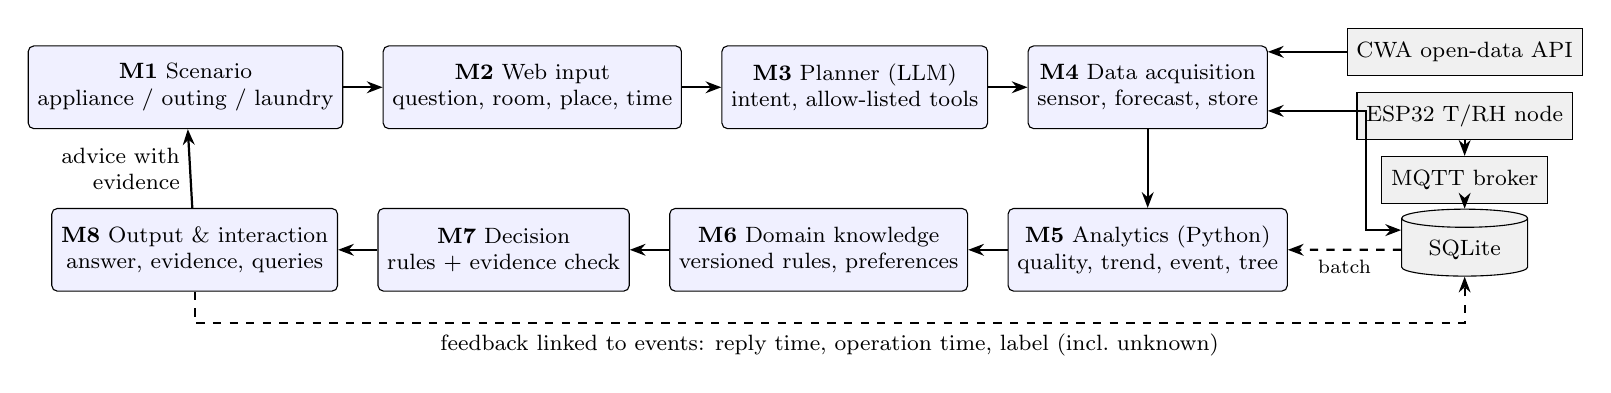
\begin{tikzpicture}[
  font=\footnotesize,
  mod/.style={draw, rounded corners=2pt, fill=blue!6, minimum width=3.0cm, minimum height=1.05cm, align=center},
  src/.style={draw, fill=gray!12, minimum width=1.9cm, minimum height=0.6cm, align=center},
  db/.style={draw, cylinder, shape border rotate=90, aspect=0.2, fill=gray!12, minimum width=1.6cm, minimum height=0.85cm, align=center},
  arr/.style={-{Stealth[length=2mm]}, thick},
  darr/.style={-{Stealth[length=2mm]}, thick, dashed},
  node distance=0.5cm and 0.5cm]
  % top row: on-demand path
  \node[mod] (m1) {\textbf{M1} Scenario\\appliance / outing / laundry};
  \node[mod, right=of m1] (m2) {\textbf{M2} Web input\\question, room, place, time};
  \node[mod, right=of m2] (m3) {\textbf{M3} Planner (LLM)\\intent, allow-listed tools};
  \node[mod, right=of m3] (m4) {\textbf{M4} Data acquisition\\sensor, forecast, store};
  % bottom row
  \node[mod, below=1.0cm of m4] (m5) {\textbf{M5} Analytics (Python)\\quality, trend, event, tree};
  \node[mod, left=of m5] (m6) {\textbf{M6} Domain knowledge\\versioned rules, preferences};
  \node[mod, left=of m6] (m7) {\textbf{M7} Decision\\rules + evidence check};
  \node[mod, left=of m7] (m8) {\textbf{M8} Output \& interaction\\answer, evidence, queries};
  % data sources column
  \node[src, right=1.0cm of m4, yshift=0.45cm] (cwa) {CWA open-data API};
  \node[src, below=0.2cm of cwa] (esp) {ESP32 T/RH node};
  \node[src, below=0.2cm of esp] (mqtt) {MQTT broker};
  \node[db] (sql) at (mqtt |- m5) {SQLite};
  % on-demand path
  \draw[arr] (m1) -- (m2);
  \draw[arr] (m2) -- (m3);
  \draw[arr] (m3) -- (m4);
  \draw[arr] (m4) -- (m5);
  \draw[arr] (m5) -- (m6);
  \draw[arr] (m6) -- (m7);
  \draw[arr] (m7) -- (m8);
  \draw[arr] (m8) -- node[left, align=right]{advice with\\evidence} (m1);
  % sources
  \draw[arr] (esp) -- (mqtt);
  \draw[arr] (mqtt) -- (sql);
  \draw[arr] (cwa.west) -- (cwa.west -| m4.east);
  \draw[{Stealth[length=2mm]}-{Stealth[length=2mm]}, thick] ($(sql.west)+(0,0.25)$) -- ++(-0.45,0) |- ($(m4.east)+(0,-0.3)$);
  % monitoring / feedback
  \draw[darr] (sql.west) -- node[below]{\scriptsize batch} (m5.east);
  \draw[darr] (m8.south) -- ++(0,-0.4) -| node[pos=0.25, below]{feedback linked to events: reply time, operation time, label (incl.\ unknown)} (sql.south);
\end{tikzpicture}
\caption{Eight-module architecture. Solid arrows: on-demand advice path. Dashed arrows: background monitoring and feedback, which link replies to events and feed versioned batch comparisons of rules and the decision tree. The LLM in M3 selects tools and explains; all numbers are computed in M5 and checked in M7.}
\label{fig:arch}
\end{figure*}

\subsection{Constrained Tool Routing}
{\sloppy
The planner may call only five tools: \texttt{get\_indoor\_state} (latest valid readings and trend features for a room), \texttt{get\_forecast} (snapshot for a township and window), \texttt{get\_device\_state} (most recent confirmed operation, or \textsc{unknown}), \texttt{get\_rules} (rules and preferences for an intent), and \texttt{log\_recommendation}. Tool arguments are validated by code before execution, and each call is logged. Following AdaHome's observation that simple commands do not need multi-step reasoning~\cite{lim2026adahome}, intents with a fixed tool set (e.g., ``current room humidity'') use a direct route, and the LLM plans only for composite questions such as laundry drying, which needs both indoor and outdoor data.\par}

\subsection{Quality Checks and Spatiotemporal Alignment}
Before analysis, each source is checked for missing values, physically implausible readings, out-of-order timestamps, gaps, and freshness. An indoor reading is fresh if $t_{\mathrm{now}}-t_i\le\Delta_{\mathrm{fresh}}$. A forecast snapshot applies to a request $(\ell^\ast, H)$ only if $\ell=\ell^\ast$ and $H\cap[v_0,v_1)\neq\emptyset$; otherwise the agent states that outdoor information is unavailable for that place and time. Indoor readings are used only for the sensed room, never as a proxy for a balcony or destination. After a communication gap, the trend window restarts, so a jump across the gap cannot create an event.

\subsection{Rule-Guided Recommendation with Evidence Check}
Table~\ref{tab:rules} lists the initial rules. Each rule has an identifier, source, version, preconditions, and stated limitations; preferences refine but cannot override quality checks. Algorithm~\ref{alg:advice} gives the advice path. If the evidence is incomplete, the agent asks for clarification or abstains (line~11). The LLM's explanation is accepted only if it is evidence-consistent; otherwise a deterministic template renders the same candidate recommendation (lines~12--13). The check extracts every number, time expression, place name, and device state from the generated text and matches it against $E$.

\begin{table}[t]
\caption{Initial Domain Rules (Version 1)}
\label{tab:rules}
\centering
\footnotesize
\setlength{\tabcolsep}{3pt}
\begin{tabular}{@{}>{\raggedright}p{0.85cm}>{\raggedright}p{2.45cm}>{\raggedright}p{2.15cm}>{\raggedright\arraybackslash}p{2.45cm}@{}}
\toprule
ID & Condition (source) & Response & Limitation \\
\midrule
DK-01 & RH persistently high; keep RH $<$60\%~\cite{epa_mold} & Adjustable dehumidification advice, given trend and device state & Reference value, not a comfort or mold diagnosis \\
DK-02 & $T$ rises while RH falls~\cite{nws_dewpoint} & Interpret $T$, RH, and $T_d$ jointly & Must not infer that a dehumidifier is on \\
DK-03 & User reports stuffiness~\cite{ashrae55,mishra2026myths} & Ask preference; general appliance advice & Air speed, radiation, clothing, activity unmeasured \\
DK-04 & Rain possible at destination and window~\cite{cwa_township} & Conditional outing / outdoor drying advice & A forecast is not observed rain \\
DK-05 & Indoor drying requested & Options combining indoor $T$/RH and ventilation & Drying time not predicted \\
\bottomrule
\end{tabular}
\end{table}

\begin{algorithm}[t]
\caption{Advice Path}
\label{alg:advice}
\small
\begin{algorithmic}[1]
\Require query $Q$, room $r$, destination $\ell^\ast$, window $H$
\Ensure advice $A$ with evidence $E$, or a clarification
\State $(\mathit{intent},\mathit{miss})\gets\textsc{Parse}(Q,r,\ell^\ast,H)$ \Comment{M2, M3}
\If{$\mathit{miss}\neq\emptyset$} \Return \textsc{AskFor}$(\mathit{miss})$ \EndIf
\State $\pi\gets\textsc{SelectAllowedTools}(\mathit{intent})$ \Comment{M3}
\State $D\gets\textsc{Fetch}(\pi,r,\ell^\ast,H)$ \Comment{M4}
\If{\textsc{InvalidStaleOrMisaligned}$(D)$} \Return \textsc{ExplainLimit}$(D)$ \EndIf
\State $X\gets\textsc{Analyze}(D)$ \Comment{M5}
\State $K\gets\textsc{GetRules}(\mathit{intent})$ \Comment{M6}
\State $S\gets\textsc{ConfirmedState}(r)$, default \textsc{unknown}
\State $C\gets\textsc{ApplyRules}(X,K,S)$ \Comment{M7}
\State $E\gets\textsc{CollectEvidence}(D,X,K)$
\If{\textsc{Incomplete}$(C,E)$} \Return \textsc{ClarifyOrAbstain}$(E)$ \EndIf
\State $A\gets\textsc{Explain}(Q,C,E)$ \Comment{M8, LLM}
\If{\textbf{not} \textsc{Consistent}$(A,E)$} $A\gets\textsc{Template}(C,E)$ \EndIf
\State \textsc{Log}$(\pi,A,E)$
\State \Return $(A,E)$
\end{algorithmic}
\end{algorithm}

\subsection{Event Detection and Feedback}
The monitoring path (Fig.~\ref{fig:flow}, Algorithm~\ref{alg:event}) operates on the most recent contiguous valid window. After smoothing with a moving average of width $w$, the slopes $\beta_T(t)$ and $\beta_\phi(t)$ are estimated by least squares over a window of length $L$. A sample is \emph{active} if
\begin{equation}
|\beta_T(t)|\ge\theta_T \;\lor\; |\beta_\phi(t)|\ge\theta_\phi ,
\label{eq:active}
\end{equation}
and a candidate event starts after $k$ consecutive active samples, so that isolated spikes are ignored. Candidates separated by less than $g$ are merged into one event. A query is sent for event $e$ only if no query for $e$ is pending and at least $\tau_{\mathrm{cd}}$ has elapsed since the last query (the cooldown). Each query has a deadline; expired queries are labeled \textsc{unk}. A reply records the reply time and the operation time separately, because residents often answer late. Residents can also log operations proactively, and ordinary periods are sampled as well, so that the dataset does not consist only of system-triggered anomalies~\cite{settles2009active}.

The parameters $(w, L, \theta_T, \theta_\phi, k, g, \tau_{\mathrm{cd}}, \Delta_{\mathrm{fresh}})$ are selected on the training period only and are stored with a version identifier; the test period is never used for tuning.

\begin{figure}[t]
\centering
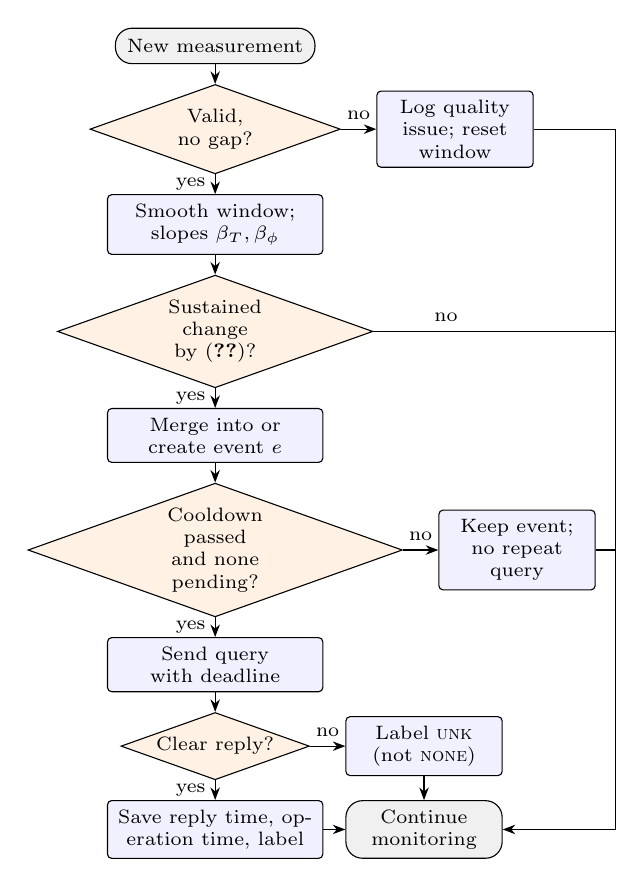
\begin{tikzpicture}[
  font=\scriptsize,
  box/.style={draw, rounded corners=1.5pt, fill=blue!6, text width=2.5cm, align=center, minimum height=0.5cm},
  side/.style={draw, rounded corners=1.5pt, fill=blue!6, text width=1.75cm, align=center, minimum height=0.5cm},
  dec/.style={draw, diamond, aspect=2.8, fill=orange!10, inner sep=0.3pt, text width=1.7cm, align=center},
  term/.style={draw, rounded corners=6pt, fill=gray!12, text width=2.3cm, align=center, minimum height=0.45cm},
  arr/.style={-{Stealth[length=1.6mm]}},
  node distance=0.25cm]
  \node[term] (start) {New measurement};
  \node[dec, below=of start] (valid) {Valid, no gap?};
  \node[box, below=of valid] (trend) {Smooth window; slopes $\beta_T,\beta_\phi$};
  \node[dec, below=of trend] (sus) {Sustained change by (\ref{eq:active})?};
  \node[box, below=of sus] (merge) {Merge into or create event $e$};
  \node[dec, below=of merge] (cool) {Cooldown passed and none pending?};
  \node[box, below=of cool] (ask) {Send query with deadline};
  \node[dec, below=of ask] (reply) {Clear reply?};
  \node[box, below=of reply] (save) {Save reply time, operation time, label};
  \node[side, right=0.45cm of valid] (q) {Log quality issue; reset window};
  \node[side, right=0.45cm of cool] (keep) {Keep event; no repeat query};
  \node[side, right=0.45cm of reply] (unk) {Label \textsc{unk} (not \textsc{none})};
  \coordinate (rail) at ($(keep.east)+(0.25,0)$);
  \node[term, text width=1.75cm] (back) at (unk |- save) {Continue monitoring};
  \draw[arr] (start) -- (valid);
  \draw[arr] (valid) -- node[left]{yes} (trend);
  \draw[arr] (trend) -- (sus);
  \draw[arr] (sus) -- node[left]{yes} (merge);
  \draw[arr] (merge) -- (cool);
  \draw[arr] (cool) -- node[left]{yes} (ask);
  \draw[arr] (ask) -- (reply);
  \draw[arr] (reply) -- node[left]{yes} (save);
  \draw[arr] (save) -- (back);
  \draw[arr] (valid) -- node[above]{no} (q);
  \draw[arr] (cool) -- node[above]{no} (keep);
  \draw[arr] (reply) -- node[above]{no} (unk);
  \draw[arr] (unk) -- (back);
  \draw (q.east) -- (q.east -| rail);
  \draw (keep.east) -- (rail |- keep.east);
  \draw (sus.east) -- node[above, pos=0.3]{no} (sus.east -| rail);
  \draw[arr] (q.east -| rail) |- (back.east);
\end{tikzpicture}
\caption{Background monitoring and feedback path. Gaps never create events, repeated queries for one event are suppressed, and missing replies are kept as unknown.}
\label{fig:flow}
\end{figure}

\begin{algorithm}[t]
\caption{Event Monitoring and Feedback}
\label{alg:event}
\small
\begin{algorithmic}[1]
\Require measurement stream $\mathcal{M}$, feedback $\mathcal{F}$, timer ticks
\Ensure event log $\mathcal{V}$, labeled events $\mathcal{Y}$
\For{each new $m\in\mathcal{M}$}
  \If{\textsc{InvalidOrGap}$(m)$} \textsc{LogAndReset}$(m)$; \textbf{continue} \EndIf
  \State $W\gets\textsc{ContiguousWindow}(m.t)$; $X\gets\textsc{Trends}(W)$
  \If{\textbf{not} \textsc{Sustained}$(X)$} \textbf{continue} \EndIf
  \State $e\gets\textsc{MergeOrCreate}(X,m.t)$
  \If{\textsc{CanAsk}$(e)$} \textsc{SendQuery}$(e)$ \EndIf
\EndFor
\For{each $f\in\mathcal{F}$}
  \State \textsc{SaveTimes}$(f.\mathit{reply\_t}, f.\mathit{op\_t})$
  \If{\textsc{Confirmed}$(f)$} \textsc{Link}$(f.e, f.\mathit{label})$
  \Else\ \textsc{Link}$(f.e, \textsc{unk})$ \EndIf
\EndFor
\For{each timer tick $t$}
  \State \textsc{ExpirePrompts}$(t)$ \Comment{expired $\Rightarrow$ \textsc{unk}}
  \If{\textsc{Scheduled}$(t)$ \textbf{and} \textsc{Enough}$(\mathcal{Y})$}
    \State $(\mathcal{D}_{tr},\mathcal{D}_{te})\gets\textsc{SplitByEventAndTime}(\mathcal{Y})$
    \State $h\gets\textsc{FitTree}(\mathcal{D}_{tr})$ \Comment{decision-time features}
    \State \textsc{CompareToRules}$(h,\mathcal{D}_{te})$; \textsc{Version}$(h)$
  \EndIf
\EndFor
\end{algorithmic}
\end{algorithm}

\subsection{Operation Identification}
The baseline is the fixed-rule detector in (\ref{eq:active}) with a rule-to-label mapping (e.g., falling $T$ with falling $T_d$ suggests \textsc{ac}; rising $T$ with falling $T_d$ suggests \textsc{dh}). The candidate model is a shallow decision tree, chosen for interpretability, using features computed only from data available at event onset: $T$, $\phi$, $T_d$, their slopes and changes over the window, time of day, and the indoor--outdoor temperature difference when a valid snapshot exists. Classification first separates operation from no operation; finer classes are added only when each has enough confirmed test events. If labels are insufficient or the tree does not outperform the rules on held-out events, the deployed system keeps the rules.

% =====================================================================
\section{Evaluation Methodology}
% =====================================================================
\subsection{Data Collection}
One room is instrumented for about two weeks. The dataset contains indoor measurements, hourly CWA snapshots for the residents' usual destinations, system-triggered queries and replies, and proactive operation logs. The UCI occupancy data~\cite{candanedo2016occupancy} are used only to test the preprocessing and plotting pipeline; its occupancy labels are not used as appliance labels.

\subsection{Leakage-Free Splitting}
Adjacent windows of one operation are highly correlated, so samples are grouped by event and split by time: the later events form the test set. No event contributes to both sets, features use only information available at decision time, and all thresholds are fixed before the test set is examined (R5).

\subsection{Experiments and Metrics}
Table~\ref{tab:eval} defines the three comparisons. For identification, we report per-class event counts, precision, recall, macro-F1, and confusion matrices; \textsc{unk} events are excluded from training and scoring and are reported separately. For interaction burden, the two policies are replayed on the same event stream: the \emph{basic} policy queries on every candidate, and the \emph{proposed} policy adds aggregation and cooldown. We report the query rate (queries per monitored hour), the reply rate (replied / sent), and the duplicate-query rate (events queried more than once / events queried). For answer quality, a fixed rule template and the LLM agent answer the same predefined scenario suite, including an appliance already on, indoor--outdoor contrast, laundry drying, API failure, and an expired snapshot. Each scenario specifies its required tools, required evidence, and acceptable answers in advance. We report tool-selection accuracy, the evidence-consistency rate, the appropriate-clarification rate on scenarios with missing or stale data, and the median and 95th-percentile end-to-end latency.

\begin{table}[t]
\caption{Evaluation Design}
\label{tab:eval}
\centering
\footnotesize
\setlength{\tabcolsep}{3pt}
\begin{tabular}{@{}>{\raggedright}p{1.9cm}>{\raggedright}p{2.35cm}>{\raggedright\arraybackslash}p{3.6cm}@{}}
\toprule
Question & Comparison & Metrics \\
\midrule
Does feedback help identification? & Fixed rules vs.\ decision tree & Events per class, precision, recall, macro-F1, confusion matrix \\
Can burden be bounded? & Basic query vs.\ aggregation + cooldown & Queries/h, reply rate, duplicate-query rate, perceived disturbance \\
Are answers evidence-based? & Rule template vs.\ LLM agent & Tool-selection accuracy, evidence consistency, appropriate clarification, latency \\
\bottomrule
\end{tabular}
\end{table}

% =====================================================================
\section{Results and Discussion}
% =====================================================================
% TODO(after experiments): replace every red placeholder below with
% measured values, and describe what the numbers show. Report class
% counts next to every metric. Do not claim the tree is better unless
% it is better on the held-out events.
\subsection{Dataset}
\todo{The deployment collected $N$ valid measurements over $D$ days from [date] to [date], with $G$ gaps totaling $H$ hours. The detector produced $E$ candidate events, of which $E_c$ were confirmed, $E_u$ remained unknown, and $E_n$ were confirmed as no operation. Class counts: \textsc{ac} $=\cdot$, \textsc{dh} $=\cdot$, \textsc{win} $=\cdot$, \textsc{mix} $=\cdot$.}

\subsection{Operation Identification}
Table~\ref{tab:res_id} compares the rules and the tree on the held-out events. \todo{Describe the result, including where each method fails, using the confusion matrices.}

\begin{table}[t]
\caption{Operation Identification on Held-Out Events}
\label{tab:res_id}
\centering
\footnotesize
\begin{tabular}{@{}lcccc@{}}
\toprule
Method & Test events & Precision & Recall & Macro-F1 \\
\midrule
Fixed rules & \tbd & \tbd & \tbd & \tbd \\
Decision tree & \tbd & \tbd & \tbd & \tbd \\
\bottomrule
\end{tabular}
\end{table}

\subsection{Interaction Burden and Answer Quality}
Table~\ref{tab:res_burden} reports the replayed query policies and the scenario-suite results. \todo{Describe the trade-off between the number of labels obtained and the query rate, and the cases in which the agent fell back to the template.}

\begin{table}[t]
\caption{Interaction Burden and Answer Quality}
\label{tab:res_burden}
\centering
\footnotesize
\setlength{\tabcolsep}{4pt}
\begin{tabular}{@{}lcc@{}}
\toprule
\multicolumn{3}{@{}l}{\textit{(a) Query policies (same event stream)}} \\
Metric & Basic & Aggregation + cooldown \\
\midrule
Queries per hour & \tbd & \tbd \\
Reply rate (\%) & \tbd & \tbd \\
Duplicate-query rate (\%) & \tbd & \tbd \\
Confirmed labels & \tbd & \tbd \\
\midrule
\multicolumn{3}{@{}l}{\textit{(b) Scenario suite ($n=$ \tbd\ scenarios)}} \\
Metric & Template & LLM agent \\
\midrule
Tool-selection accuracy (\%) & \tbd & \tbd \\
Evidence consistency (\%) & \tbd & \tbd \\
Appropriate clarification (\%) & \tbd & \tbd \\
Latency, median / p95 (s) & \tbd & \tbd \\
\bottomrule
\end{tabular}
\end{table}

\subsection{Limitations}
The study covers one room, one sensor, and about two weeks, so the results characterize this setting and do not generalize across households or seasons. Temperature and RH alone cannot establish thermal comfort, because air speed, radiant temperature, clothing, and activity are not measured~\cite{ashrae55}; the agent therefore reports these as unmeasured factors. Self-reports may be delayed or uncertain, which is why reply and operation times are stored separately and uncertain replies are kept as unknown. Township forecasts describe a representative point and window, not the user's exact location~\cite{cwa_township}. Finally, the system does not control appliances, optimize energy, or predict laundry drying time; these are left for future work.

% =====================================================================
\section{Conclusion}
% =====================================================================
% TODO(after experiments): add one or two sentences stating the main
% measured findings.
This paper presented an evidence-traceable domain-specific agent that combines single-room temperature--humidity sensing, township forecasts, versioned rules, and user feedback to support everyday decisions about appliances, outings, and laundry drying. The design keeps computation in code and limits the LLM to intent parsing, tool routing, and explanation, binds every recommendation to an evidence record, and degrades to clarification, abstention, or a template when data or explanations cannot be verified. Its event-triggered feedback loop collects time-aligned operation labels under an explicit query cooldown and keeps unknown and mixed operations distinct. The event-grouped temporal protocol makes it possible to quantify the trade-off between identification reliability and interaction burden. Future work will extend the study to multiple rooms and seasons, add air-speed and radiant-temperature sensing, and examine closed-loop appliance control.

% \section*{Acknowledgment}
% \todo{Funding / course acknowledgment, if any.}

\bibliographystyle{IEEEtran}
\bibliography{references}

\end{document}
